%%%%%%%%%%%%%%%%%%%%%%%%%%%%%%%%%%%%%%%%%%%%%%
% An example of a lab report write-up.
%%%%%%%%%%%%%%%%%%%%%%%%%%%%%%%%%%%%%%%%%%%%%%
% This is a combination of several labs that I have done in the past for
% Computer Engineering, so it is not to be taken literally, but instead used as
% a great starting template for your own lab write up.  When creating this
% template, I tried to keep in mind all of the functions and functionality of
% LaTeX that I spent a lot of time researching and using in my lab reports and
% include them here so that it is fairly easy for students first learning LaTeX
% to jump on in and get immediate results.  However, I do assume that the
% person using this guide has already created at least a "Hello World" PDF
% document using LaTeX (which means it's installed and ready to go).
%
% My preference for developing in LaTeX is to use the LaTeX Plugin for gedit in
% Linux.  There are others for Mac and Windows as well (particularly MikTeX).
% Another excellent plugin is the Calc2LaTeX plugin for the OpenOffice suite.
% It makes it very easy to create a large table very quickly.
%
% Professors have different tastes for how they want the lab write-ups done, so
% check with the section layout for your class and create a template file for
% each class (my recommendation).
%
% Also, there is a list of common commands at the bottom of this document.  Use
% these as a quick reference.  If you'd like more, you can view the "LaTeX Cheat
% Sheet.pdf" included with this template material.
%
% (c) 2009 Derek R. Hildreth <derek@derekhildreth.com> http://www.derekhildreth.com
% This work is licensed under the Creative Commons Attribution-NonCommercial-ShareAlike License. To view a copy of this license, visit http://creativecommons.org/licenses/by-nc-sa/1.0/ or send a letter to Creative Commons, 559 Nathan Abbott Way, Stanford, California 94305, USA.
%%%%%%%%%%%%%%%%%%%%%%%%%%%%%%%%%%%%%%%%%%%%%%

\input kvmacros % For Karnaugh Maps (K-Maps)
\documentclass[UTF8]{ctexart}
\usepackage{graphicx} % For images
\usepackage{float}    % For tables and other floats
\usepackage{verbatim} % For comments and other
\usepackage{amsmath}  % For math
\usepackage{amssymb}  % For more math
\usepackage{fullpage} % Set margins and place page numbers at bottom center
\usepackage{listings} % For source code
\usepackage{subfig}   % For subfigures
\usepackage[usenames,dvipsnames]{color} % For colors and names
\usepackage{hyperref}           % For hyperlinks and indexing the PDF
\hypersetup{ % play with the different link colors here
    colorlinks,
    citecolor=blue,
    filecolor=blue,
    linkcolor=blue,
    urlcolor=blue % set to black to prevent printing blue links
}

\definecolor{mygrey}{gray}{.96} % Light Grey
\lstset{
	language=[ISO]C++,              % choose the language of the code ("language=Verilog" is popular as well)
   tabsize=3,							  % sets the size of the tabs in spaces (1 Tab is replaced with 3 spaces)
	basicstyle=\tiny,               % the size of the fonts that are used for the code
	numbers=left,                   % where to put the line-numbers
	numberstyle=\tiny,              % the size of the fonts that are used for the line-numbers
	stepnumber=2,                   % the step between two line-numbers. If it's 1 each line will be numbered
	numbersep=5pt,                  % how far the line-numbers are from the code
	backgroundcolor=\color{mygrey}, % choose the background color. You must add \usepackage{color}
	%showspaces=false,              % show spaces adding particular underscores
	%showstringspaces=false,        % underline spaces within strings
	%showtabs=false,                % show tabs within strings adding particular underscores
	frame=single,	                 % adds a frame around the code
	tabsize=3,	                    % sets default tabsize to 2 spaces
	captionpos=b,                   % sets the caption-position to bottom
	breaklines=true,                % sets automatic line breaking
	breakatwhitespace=false,        % sets if automatic breaks should only happen at whitespace
	%escapeinside={\%*}{*)},        % if you want to add a comment within your code
	commentstyle=\color{BrickRed}   % sets the comment style
}

% Make units a little nicer looking and faster to type
\newcommand{\Hz}{\textsl{Hz}}
\newcommand{\KHz}{\textsl{KHz}}
\newcommand{\MHz}{\textsl{MHz}}
\newcommand{\GHz}{\textsl{GHz}}
\newcommand{\ns}{\textsl{ns}}
\newcommand{\ms}{\textsl{ms}}
\newcommand{\s}{\textsl{s}}



% TITLE PAGE CONTENT %%%%%%%%%%%%%%%%%%%%%%%%
% Remember to fill this section out for each
% lab write-up.
%%%%%%%%%%%%%%%%%%%%%%%%%%%%%%%%%%%%%%%%%%%%%

\newcommand{\labtitle}{大作业}
\newcommand{\authorname}{李梓铉}
\newcommand{\professor}{张选平教授}
\newcommand{\classno}{3118103163}
% END TITLE PAGE CONTENT %%%%%%%%%%%%%%%%%%%%


\begin{document}  % START THE DOCUMENT!


% TITLE PAGE %%%%%%%%%%%%%%%%%%%%%%%%%%%%%%%%%%%%%%
% If you'd like to change the content of this,
% do it in the "TITLE PAGE CONTENT" directly above
% this message
%%%%%%%%%%%%%%%%%%%%%%%%%%%%%%%%%%%%%%%%%%%%%%%%%%%
\begin{titlepage}
\begin{center}
{\LARGE \textsc{算法分析与复杂性理论:} \\ \vspace{4pt}}
{\Large \textsc{\labtitle} \\ \vspace{4pt}}
\rule[13pt]{\textwidth}{1pt} \\ \vspace{150pt}
{\large  \authorname \\ \vspace{10pt}
学号 \classno\\ \vspace{10pt}
指导老师: \professor \\ \vspace{10pt}
\today}
\end{center}
\end{titlepage}
% END TITLE PAGE %%%%%%%%%%%%%%%%%%%%%%%%%%%%%%%%%%





%%%%%%%%%%%%%%%%%%%%%%%%%%%%%%
%%%%%%%%%%%%%%%%%%%%%%%%%%%%%%
\section{复杂度问题}
%No Text Here
%%%%%%%%%%%%%%%%%%%%%%%%%%%%%%%
\subsection{题目}
\begin{comment}
This is a lab template which has a ton of different things which are useful in writing lab write-ups in the Computer Eningeering field.  This is demonstrating the comment block. Don't be overwhelmed, it may seem like a lot to take in at a time, but it's worth spending the time learning it.
\end{comment}
已知$\mathrm{T}(\mathrm{n}) \leq \left\{\begin{array}{cl}{c_{1}} & {n \leq 1} \\ {\max (T(i)+T(n-i-1))+c_{2} n} & {n>1}\end{array}\right.,(1<=i<=\mathrm{n}-1)
,其中c_{1},c_{2}$,为正常数,请证明$\mathrm{T}(\mathrm{n})=\Theta\left(\mathrm{n}^{2}\right)$。
\vspace{3mm}

\begin{comment}
\begin{itemize}
	\item 主成分分析方法(PCA)
	\item 核主成分分析方法(KPCA)
	\item 局部性嵌入(LLE)
	\item 工程应用
	\item 结论与讨论
\end{itemize}
\vspace{3mm}
\end{comment}
%%%%%%%%%%%%%%%%%%%%%%%%%%%%%%
\subsection{证明}
令T(n)对应最坏情况的时间则
\begin{equation}
  T(n)={\max (T(i)+T(n-i-1))+c_{2} n}
\end{equation}
假设对于任何k<n,总有$T(k) \leq c{k}^{2}$ 其中c为常数,显然k=1时成立。将归纳假设带入(1)式可以得到:
\begin{equation}
  T(n)\leq{c\max ({i}^{2}+{(n-i-1)}^{2}))+c_{2} n}
\end{equation}

显然在[1,n-1]上,i=1或n-1时取最大值${(n-2)}^{2}+1$ 于是有:
\begin{equation}
  T(n)\leq{c{n}^{2}+c(5-4n)+c_{2}n}\leq c{n}^{2}
\end{equation}
因为n>=2,所以只要c足够大,第二个等号就成立。因此有$T(n)<=cn^{2}$. 根据归纳法,k成立则n成立,且k=1时成立。所以对于所有的n都有$T(n)<=cn^{2}$. 得证


%%%%%%%%%%%%%%%%%%%%%%%%%%%%%%
%\subsection{Procedure}

%	\begin{enumerate}
%		\item Start the ISE Navigator. See the ISE 8.2i Quick Start Tutorial.
%		\item Create a new project.
%		\item Import copies of the Verilog modules AND\_OR, MY\_AND2, and MY\_OR2 to the new project just created.
%		\item Create a Test Bench (called Test Fixture in Verilog).
%		\item Create the actual input stimulus.
%		\item Run the simulation, examine the waveforms, and verify functioniality.
%	\end{enumerate}

%%%%%%%%%%%%%%%%%%%%%%%%%%%%%%
%%%%%%%%%%%%%%%%%%%%%%%%%%%%%%
\newpage
\section{凸包问题}
\subsection{题目}
给定平面上 n 个点,从中找出一个最小点集,使该点集所组成的凸多边形包围所有的 n 个点。用分治法编写一个求解凸包问题的算法。

\subsection{算法设计}

首先想一个可行的暴力算法,依次取点集n中所有可能的边$C_n^2$,每取一条边,遍历其他所有点判断是否都在该边的上方或下方。满足条件即为凸包的一条边。该算法复杂度易得是$O(n^3)$。 使用分治法,将点集按横坐标顺序从左到右排序(nlogn)均分为每个含有五个点的点集。可知每个子集只有限次搜索即可得到子集的凸集,找到所有子集的凸集的时间复杂度为$O(n)$。此时再用一个巧妙地方法将子集凸包合并起来即可。相邻凸包的左边凸包的最右点与右边凸包的最左点作为初始点对,不妨先选左边凸包为调整对象。在点集中依横坐标减小顺序向左搜索纵坐标大于最右点的点,直到该点连线与左边凸包相切(每判断一次相切至需要子凸包的点数n'次),同理再调整右边凸包的点,直到找到上方的公共切线。下方切线同理。显然点数有限,每两个凸包合并时间复杂度即为O(n)。将合并的凸包与该凸包右边的子凸包继续合并,就可得到原点集的凸包,合并的时间复杂度为$O(n^2)$。因此算法复杂度为$nlogn+O(n)+O(n^2)=O(n^2)$。	\vspace{3mm}

算法的主要过程总结如下:
\begin{enumerate}
	\item 输入:包含n个点的点集
	\item 将点集根据横坐标顺序排序
	\item 按顺序每五个点作为一个子点集进行划分
	\item 在每个子点集中使用暴力枚举得到子集的凸包
	\item 寻找相邻子集凸包的上下两条切线连接的点
  \item 合并所有子集的凸包
	\item 输出:点集的凸包
\end{enumerate}


\subsection{测试实例}
使用python语言实现了一个个数为9的点集的求解,但包含了算法中所有的关键步骤如暴力求解部分,寻找切线部分,和合并部分都在。如果求解大于10的个数的点集还做不到完全的自动化,还需要修改,但由于是算法作业,在验证算法可行性上已经足够。下面是测试结果:

	\begin{figure}[H]
	  \centering
	  \label{fig:Per6A}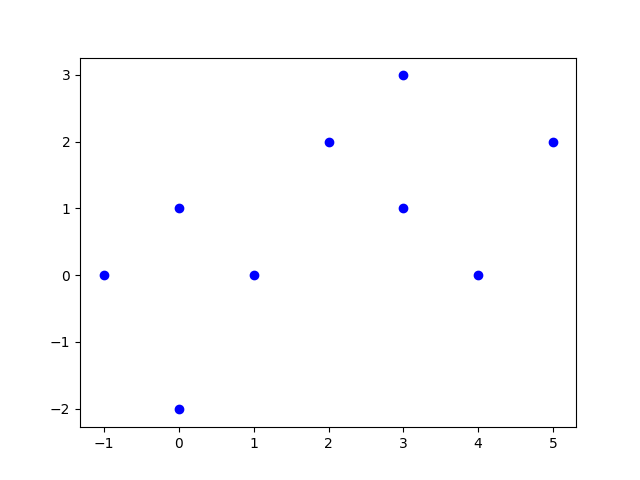
\includegraphics[width=0.4\textwidth]{original.png}\
	  \caption{原始点集}
	  \label{fig:oscil}
	\end{figure}

  \begin{figure}[H]
    \centering
    \label{fig:Per6A}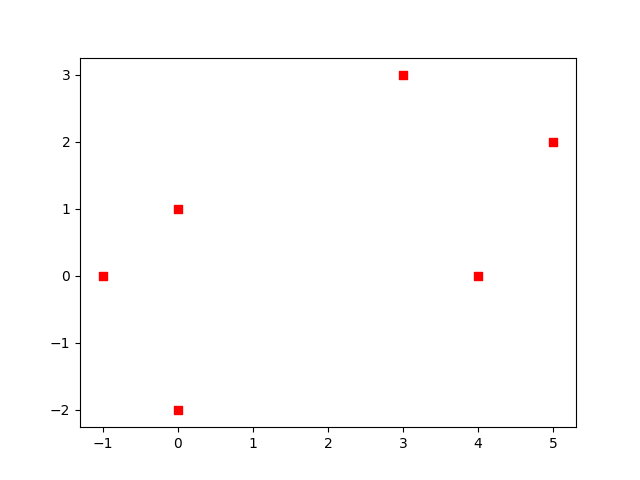
\includegraphics[width=0.4\textwidth]{convex.png}\
    \caption{求解得到的凸包}
    \label{fig:oscil}
  \end{figure}

\subsection{源代码}
实验源代码如下.  \vspace{5mm}
	\lstinputlisting{convex.py}
	\vspace{3mm}






\newpage
\section{动态规划算法}
\subsection{问题}
设计一个动态规划算法,找到字符串 T[1..n]中前向和后项相同的最长连续子串。前向子串和后项子串不能重叠。例如:
\begin{enumerate}
  \item 输入“ALGORITHM”,算法返回空串;
  \item 输入“RCURSION”,算法返回“R”;
  \item 输入“REDIVIDE”,算法返回“EDI”。
\end{enumerate}

\subsection{算法设计}
最差情况下要找到最大子串显然所有字符都要比较至少一次才能确保找到最大字符串,考虑动态规划的算法思路,比较字符是否相同显然是相关子问题被重复计算了很多次。如果能够保存已解决的子问题的答案,而在需要时再找出已求得的答案,这样就可以避免大量的重复计算,节省时间。所以我用一个表来记录所有已解的子问题的答案。先将字符串反向排列作为一个二维矩阵的纵向指标,再将原字符串作为二维矩阵的横向指标。再开始填写表,如果横纵指标相同,且字符不是翻转前后的同一个字符,那么该空填为1,否则填为0,完整的填写需要$n^2$次,图3给出了该部分的示意图。

\begin{figure}[H]
  \centering
  \label{fig:Per6A}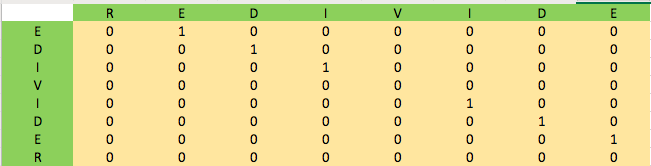
\includegraphics[width=0.8\textwidth]{lcs.png}\
  \caption{表格示意图}
  \label{fig:oscil}
\end{figure}

然后将矩阵从左下角到右上角对角遍历循环输出便可得到所有可能的对称子串,如图4所示。找出其中1个数最多的子串即为前向后向相同的最长连续子串,至多需要2n-1次。所以算法复杂度为$O(n^2)$

\begin{figure}[H]
  \centering
  \label{fig:Per6A}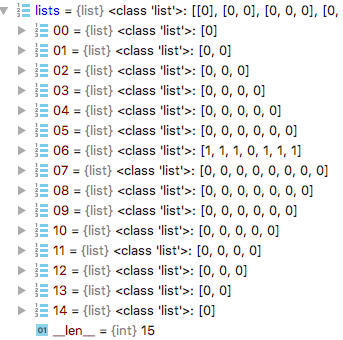
\includegraphics[width=0.5\textwidth]{list.png}\
  \caption{对角遍历输出}
  \label{fig:oscil}
\end{figure}
\vspace{3mm}

算法的主要过程可以总结如下:

\begin{enumerate}
	\item 输入:字符串T[1..n]$\phi$
	\item 得到字符串反向排列
	\item 填写比较表格
  \item 对角遍历输出所有可能的对称子串,找到对称最长连续子串对应的字母对应的位置
	\item 输出:最长连续子串
\end{enumerate}


\subsection{测试示例}
以题目给的三个例子,输入“ALGORITHM”,算法返回空串;输入“RCURSION”,算法返回“R”;输入“REDIVIDE”,算法返回“EDI”,作为测试,并且测试很多其他例子,都没有问题。下面是测试结果。
\begin{figure}[H]
  \centering
  \label{fig:Per6A}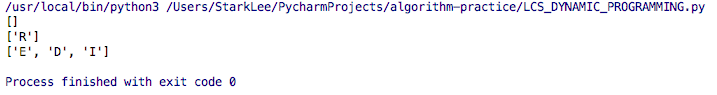
\includegraphics[width=0.8\textwidth]{result2.png}\
  \caption{返回的最长连续子串}
  \label{fig:oscil}
\end{figure}

\subsection{源代码}
实验源代码如下.  \vspace{5mm}
	\lstinputlisting{LCS_DYNAMIC_PROGRAMMING.py}
	\vspace{3mm}




\newpage
\section{贪心算法}
\subsection{问题}
假定 J={1,2,3,...,n}是 n 个等待在同一台机器上加工的作业集合,每个作业所需要的加工时间都为 1 个时间单位,且每个作业 i 都有一个最迟完成时间 di。如果一个作业 i 能够在 di 之前完成,就可获得收益 pi>0;反之,则不获得收益。请设计一个贪心的算法求该问题的一个最佳安排方案使得收益最大,并证明你所设计的贪心策略的最优性。\vspace{3mm}



\subsection{算法设计}
贪心算法在每一部做出局部最优的选择,并寄希望于这样的选择可以得到全局最优。对于题目,如果在截止时间后完成,任务称为延迟,如果在截止时间前完成,称为提前的。 对于任意一个安排方案都可以以提前优先的形式,即将提前的任务都放在延迟任务之前,并将提前任务然截止时间单调递增的顺序排列。如果存在一个任务集合,有调度方案使得所有任务都不延迟,则称该任务是独立的。 原问题及转换为寻找最优独立提前子任务集。 较为显然对于任意的有n个元素的独立任务集合有,t在[1...n]时,集合中截止时间小于t的任务数量一定小于t(因为大于的话一定会发生延迟)。 因此贪心算法设计思路就是,优先选择收益最大的作业,并每选择一个作业后验证更新之后的任务集合仍然满足独立条件。每次验证独立性的时间复杂度为O(nlogn),又需要进行n次独立性验证,因此时间复杂度为$O(n^2logn)$


算法的主要过程可以总结如下:
\begin{enumerate}
	\item 输入:任务集$D={x_1,x_2,...,x_m}$,
  \item 对任务集根据奖励价值由高到低进行排列
	\item for i = 1,2,...,m do
	\item 对于集合fin 增加任务集中的第i个元素
	\item 检验集合fin 的独立性
	\item if 不满足独立性,删除掉该元素
	\item endif
	\item endfor
	\item 输出:最优的安排方案
\end{enumerate}

最优性证明:如果S是一个给定截止时间的单位时间任务集合,$\mathcal{I}$ 是所有独立任务集合的集合,则对应的系统$S,\mathcal{I}$可以证明是一个拟阵:假设B和A是独立的任务集合,且$|B|>|A|$.取k是满足$N_{t}(B) \leqslant N_{t}(A)$ 最大的t。因为$N_{n}(B)=|B|$ 且 $N_{n}(A)=|A|$ 但|$B|>|A|$。因此对任意j: $k+1 \leq j \leq n$,必然有k<n且$N_{j}(B)>N_{j}(A)$,因此B比A包含更多截止时间为k+1的任务。令ai为B-A中截止时间为k+1的任务,令
$A^{\prime}=A \cup\left\{a_{i}\right\}$
,和之前证明独立一样,较为显然对于任意的有n个元素的独立任务集合有,t在[1...n]时,集合中截止时间小于t的任务数量一定小于t(因为大于的话一定会发生延迟),易得A'必然也是独立的。而对于$0\leq k \leq n$ 有 $N_{t}\left(A^{\prime}\right)=N_{t}(A) \leqslant t$.所以A'独立,所以$S,\mathcal{I}$是一个拟阵。而拟阵具有贪心选择性质,即如果某个元素初始不是最优的选择,那么在随后也不会选入最优集合,这保证了删除掉元素的正确性,而由于拟阵的最优子结构性质,寻找fin的最大权重独立子集并将它扩展,总体效果就是找到原集合的一个最大权重子集。


\subsection{测试示例}
输入任务集合d = [(70,4), (60,2), (50,4), (40,3), (30,1), (20,4), (10,6)] 第一项为奖励,第二项为截止时间。
最优解将会舍弃(30,1)与(20,4)两个任务。

\begin{figure}[H]
  \centering
  \label{fig:Per6A}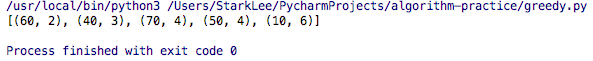
\includegraphics[width=0.8\textwidth]{result3.png}\
  \caption{最优任务安排}
  \label{fig:oscil}
\end{figure}

算法得到了最优解,实现验证。

\subsection{源代码}
实验使用的源代码如下.  \vspace{5mm}
	\lstinputlisting{greedy.py}
	\vspace{3mm}




\newpage
\section{集合覆盖问题}
\subsection{问题}
给定一个集合$\mathrm{X}=\left\{x_{1}, x_{2}, \ldots x_{n}\right\}$ 以及 X 的一个子集簇 $\mathrm{F}=\left\{f_{1}, f_{2}, \ldots, f_{n}\right\}$,其中,$f_{i} \subseteq X$。求F的一个最小子集C,使得C中的集合能够覆盖集合X,即$(U_{S \in C} S=X)$, 完成以下两个问题

1)已知图的顶点覆盖问题是 NPC,证明集合覆盖问题是 NP 难的;

2)利用回溯法或分支界限法设计求解集合覆盖问题的算法。

\subsection{证明}
首先证明集合覆盖问题是一个np问题:显然,证书为一个F的一个子集,对于一个给定的子集验证是否能覆盖集合X,只需要多项式时间,只需将元素挨个比较即可,即集合覆盖问题是一个np问题。

下面证明顶点覆盖问题可以规约到集合覆盖问题:对于一个顶点覆盖实例G=(V,E). S=E,对于$\forall v_{i} \in V$,与vi 相连的边可以组成一个E的子边集$c_{i}$,和C对应。显然规约时间是多项式时间。

假设有一个大小至少为k的顶点覆盖A,则A的每个顶点都可以对应一个集合C的元素组成集合C',因为A是顶点覆盖,因次覆盖了所有的边,所以$\bigcup_{c \in C'} c=S$, 且$\left|C^{\prime}\right| \leq k$

假设有C的子集C',且$\left|C^{\prime}\right| \leq k$ 且 $\bigcup_{c \in C'} c=S$,因为C’的每个元素代表了G中与某个顶点相连的边,因此C'元素对应的顶点组成集合A,且一定可以覆盖G中全部的边,又因为$\left|C^{\prime}\right| \leq k$,因此A即为G的至多为k的顶点覆盖。

因此顶点覆盖问题可以在多项式时间规约到集合覆盖问题,又因为已知图的顶点覆盖问题是NPC问题,所以集合覆盖问题是NP hard的。

\subsection{算法设计}
使用分支界限法,将集合簇F中的元素按所含元素分类,写函数:首先含有$x_{1}$的作为一类,不妨以$x_{1}$类作为开始节点,每次选出类中的一个子集合,根据子集和中的元素(如含有$x_{1},x_{2}$),就排除不需要的类(如$x_{1},x_{2}$类),递归调用自己,直到所有类均被排除,即找到了可行解。可行记录可行解对应的子集簇的元素个数。并在之后搜索中将大于当前最优解的节点直接排除。直到或节点表为空即遍历了$x_{1}$中的元素之后。即得到了集合X的覆盖。
但是程序设计上,由于递归调用要求递归的任务数是不断减少的,而根据算法设计,递归的任务数是不断增加的,因此程序设计尝试了很久都没有实现。所以本节没有包含代码。但觉得NPC的问题程序设计还不如直接穷举简洁,而算法复杂度上实际差别是不大的。



\newpage
\section{结论与讨论}


最后感谢张教授这学期的教学,让我收获很多。只是有些可惜课时太少,很希望未来算法分析这门课可以调整成全周的课程。顺颂时祺。

\end{document} % DONE WITH DOCUMENT!






% IF YOU'D RATHER TYPE THE CODE, OR HAVE A SMALLER BLOCK OF CODE, USE THIS:
%\begin{lstlisting}
%if(something)
%	do this
%else
%	do this
%\end{lstlisting}

%% THIS IS FROM A DIFFERENT CLASS, BUT DEMONSTRATES MATH MODE WELL
%%%%%%%%%%%%%%%%%%%%%%%%%%%%%%
\subsection{Formulas and Overall Descriptions Used}
This part of the laboratory was done for \href{http://www.byui.edu/catalog/2004-2005/class.asp1075.htm}{Feedback Control}.  Most of this laboratory's calculations were completed and compiled by the folks at Quanser (the manufacturer of the inverted pendulum) and will give the lab a good starting place.  Below are the state equation and gain values used initially in the lab:
	\[
	\begin{bmatrix}
	\dot{\alpha} \\
	\ddot{\alpha} \\
	\dot{\theta} \\
	\ddot{\theta} \\
	\end{bmatrix}
	=
	\begin{bmatrix}
	0 & 1 & 0 & 0 \\
	81.7 & 0 & 0 & -13.9 \\
	0 & 0 & 0 & 1 \\
	39.7 & 0 & 0 & -14.4 \\
	\end{bmatrix}
	\begin{bmatrix}
	\alpha \\
	\dot{\alpha} \\
	\theta \\
	\dot{\theta} \\
	\end{bmatrix}
	+
	\begin{bmatrix}
	0 \\
	24.5 \\
	0 \\
	25.4 \\
	\end{bmatrix}
	V
	\]

	\[
	K  =
	\begin{bmatrix}
	21 & 2.8 & -2.2 & -2.0 \\
	\end{bmatrix}
	\]

Other values, such as the $\frac{\mbox{Volts}}{\mbox{Degree}}$ and $\frac{\mbox{Degrees}}{\mbox{Volt}}$ were obtained by first determining the max angle of the pendulum on both extreme sides.

Using the max angles from above, these values were determined:
	\[
	\begin{array}{l l}
		\alpha = 0.062 \frac{\mbox{Volts}}{\mbox{Degree}} \\ \\
		\alpha = 15.105 \frac{\mbox{Degrees}}{\mbox{Volt}} \\
	\end{array}
	\]

I would also like to add that in order to calibrate $\alpha$ to get a perfect vertical $= 0$, a value of $0.09$ needed to be added.  The same applies to $\theta$ where $0.322$ needs to be added.

%%%%%%%%%%%%%%%%%%%%%%%%%%%%%%
\subsection{DC Motor Transfer Function and Parameters}

Definitions:
	\begin{align*}
		\theta(t) =  Angular Position \\
		\dot{\theta}(t) =  Angular Velocity \\
		\triangle t = t_{10\%} - t_{90\%} \\
		90\% = e^{-t_{10\%}/\tau} \\
		10\% = e^{-t_{90\%}/\tau} \\
	\end{align*}

The Math:
	\begin{align*}
		\frac{s\theta(s)}{V_{a}(s)} = \frac{K}{s+P} \\
		\mbox{Let}\ V_{a}(s) = \frac{V_{0}}{s} \\  % If you'd like to have a space following any command, add "\" to the end as shown here.
		s\theta(s) = \frac{KV_{0}}{(S+P)S} = \frac{KV_{0}}{\frac{P}{S}} - \frac{\frac{KV_{0}}{P}}{s+P} \\
		L^{-1} \Rightarrow \dot{\theta}(t) = \frac{KV_{0}}{P}(1-e^{-t/(1/P)}) \\
		\dot{\theta}(t) = (\dot{\theta}_{i} - \dot{\theta}_{f})e^{-pt} + \dot{\theta}_{f} \\
	\end{align*}

Final equations:
	\begin{align}
		\label{thetadot}\dot{\theta}_{f} = \frac{KV_{0}}{P} \\
		\label{equ:tau}\frac{1}{P} = \tau = \frac{\triangle t}{ln(9)}
	\end{align}

Graphically (Refer to Equation \ref{thetadot} and Equation \ref{equ:tau}) :
	% Drawn and exported to png using Inkscape.
	\begin{figure}[h]
		\begin{center}
			\includegraphics[width=0.33\textwidth]{graph.png}
		\end{center}
	\label{graph}
	\end{figure}

% AGAIN, ANOTHER EXAMPLE FROM A DIFFERENT CLASS WHICH DEMONSTRasdATES KMAPS AND TABLES NICELY.
\newpage % I added this after viewing the completed pdf and decided to make this cosmetic change
This section consists of tables and reductions which were used in this laboratory exercise.

% This table was generated using the Calc2LaTeX macro which I mentioned earlier.
% You'll need OpenOffice installed and you'll have to download the macro online.
% If you're interested, I have a guide on how to set this up and use it on my
% blog.  http://www.derekhildreth.com/blog  Search for "LaTeX".  You'll find it.
	\begin{table}[htbp]
	\begin{center}
		\begin{tabular}{|ccc|cc|}
			\hline
			\textbf{PS} & \textbf{D} & \textbf{N} & \textbf{NS} & \textbf{P} \\ \hline
			\$0.00 & 0 & 0 & \$0.00 & 0 \\
			 & 0 & 1 & \$0.05 & 0 \\
			 & 1 & 0 & \$0.10 & 0 \\
			 & 1 & 1 & -- & -- \\ \hline
			\$0.05 & 0 & 0 & \$0.05 & 0 \\
			 & 0 & 1 & \$0.10 & 0 \\
			 & 1 & 0 & \$0.15 & 0 \\
			 & 1 & 1 & -- & -- \\ \hline
			\$0.10 & 0 & 0 & \$0.10 & 0 \\
			 & 0 & 1 & \$0.15 & 0 \\
			 & 1 & 0 & \$0.15 & 0 \\
			 & 1 & 1 & -- & -- \\ \hline
			\$0.15 & -- & -- & \$0.15 & 1 \\ \hline
			\end{tabular}
	\end{center}
	\caption{Symbolic Transition Table}
	\label{symbolic}
	\end{table}

	\begin{table}[H]
		\centering
		\subfloat[D1 = $Q_{1}$+D+$Q_{0}$N] % Caption
			{
				\karnaughmap{4}{D1:}{ {$Q_{1}$} {$Q_{0}$} {D} {N} }{001X011X111X111X}{}  % See the included kvdoc.pdf file for more details
			} \hspace{10mm} % seperate them a bit
		\subfloat[D0 = $\Bar{Q_{0}}$N + $Q_{0}\Bar{N}$ + $Q_{1}$N + $Q_{1}$D] % Caption
			{
				\karnaughmap{4}{D0:}{ {$Q_{1}$} {$Q_{0}$} {D} {N} }{010X101X011X111X}{}
			}
	  \caption{Karnaugh maps and the simplified results of the logic.}
	  \label{fig:kmaps}
	\end{table}


%%%%%%%%%%%%%%%%%%%%%%%%%%%%%%
%%%%%%%%%%%%%%%%%%%%%%%%%%%%%%
\newpage
\section{Discussion \& Conclusion}
The goal of this lab was to re-design the LED/Switch system to include a hardware timer.  By pressing eight different combinations of the three buttons, the LEDs on the board were to act in different ways using these timers. There was not a Q\&A requirement for this lab. \vspace{3mm} % I use this to seperate the paragraphs a bit.

I was able to accomplish the requirements of the lab by utilizing the \texttt{IntMgrTimerExample.c} project found within the analog devices example programs folder (and mentioned in the class lecture).  There were some stumbling blocks to overcome.  The most difficult for myself was actually getting the period of the LEDs just right.  I was able to get it very close to the 333.3\ms, 666.7\ms, and 1\s periods, but not exactly.  My first method of getting these periods right was to take the clock speed in \MHz, find the period by taking the inverse of the clock speed, and then solving for the value in hex that was needed to get the right period.  This didn't yeild very accurate results at all, and so I then went through a trial and error session until I got a value of 1.1\ms.  I used this value in hex to calculate the other periods.  The results of this method can be seen in Figure \ref{fig:oscil} above in the schematics section. \vspace{3mm}

Another observation I would like to point out is that I put all of my logic within the interrupts themselves.  I feel that this was a hacked way of doing the lab to save time and that it's probably not the best programming method.  After I was completed with my lab, I viewed other students solutions and they just seemed more elegant.  Interestingly enough, the other students weren't incredibly happy with their solution either.  If I were to go back and do this lab again, I would invest more time in both understanding how to utilze the interrupts as well as find a more elegant solution to blink the lights. \vspace{3mm}

All in all, this laboratory gave me an insight on how interrupts work and I hope to be able to apply them to following labs\ldots


\end{document} % DONE WITH DOCUMENT!


%%%%%%%%%%
PERSONAL FAVORITE LAB WRITE-UP STRUCTURE
%%%%%%%%%%
\section{Introduction}
	% No Text Here
	\subsection{Purpose}
		% Lab objective
	\subsection{Equipment}
		% Any and all equipment used (specific!)
	\subsection{Procedure}
		% Overview of the procedure taken (not-so-specific!)
\newpage
\section{Schematic Diagrams}
	% Any schematics, screenshots, block
   % diagrams used.  Possibly photos or
	% images could go here as well.
\newpage
\section{Experiment Data}
	% Depending on lab, program code would be
	% included here without the Estimated and
	% Actual Results.
	\subsection{Estimated Results}
		% Calculated. What it should be.
	\subsection{Actual Results}
		% Measured.  What it actually was.
\newpage
\section{Discussion \& Conclusion}
	% 3 Paragraphs:
		% Restate the objective of the lab
		% Discuss personal trials, errors, and difficulties
		% Conclude the lab


%%%%%%%%%%%%%%%%
COMMON COMMANDS:
%%%%%%%%%%%%%%%%
% IMAGES
begin{figure}[H]
   \begin{center}
      \includegraphics[width=0.6\textwidth]{RTL_SCHEM.png}
   \end{center}
\caption{A screenshot of the RTL Schematics produced from the Verilog code.}
\label{RTL}
\end{figure}

% SUBFIGURES IMAGES
\begin{figure}[H]
  \centering
  \subfloat[LED4 Period]{\label{fig:Per4}\includegraphics[width=0.4\textwidth]{period_led4.png}} \\
  \subfloat[LED5 Period]{\label{fig:Per5}\includegraphics[width=0.4\textwidth]{period_led5.png}}
  \subfloat[LED6 Period]{\label{fig:Per6}\includegraphics[width=0.4\textwidth]{period_led6.png}}
  \caption{Period of LED blink rate captured by osciliscope.}
  \label{fig:oscil}
\end{figure}

% INSERT SOURCE CODE
\lstset{language=Verilog, tabsize=3, backgroundcolor=\color{mygrey}, basicstyle=\small, commentstyle=\color{BrickRed}}
\lstinputlisting{MODULE.v}

% TEXT TABLE
\begin{table}
\begin{center}
\begin{tabular}{|l|c|c|l|}
	x & x & x & x \\ \hline
	x & x & x & x \\
	x & x & x & x \\ \hline
\end{tabular}
\caption{Caption}
\label{label}
\end{center}
\end{table}

% MATHMATICAL ENVIRONMENT
$ 8 = 2 \times 4 $

% CENTERED FORMULA
\[  \]

% NUMBERED EQUATION
\begin{equation}

\end{equation}

% ARRAY OF EQUATIONS (The splat supresses the numbering)
\begin{align*}

\end{align*}

% NUMBERED ARRAY OF EQUATIONS
\begin{align}

\end{align}

% ACCENTS
\dot{x} % dot
\ddot{x} % double dot
\bar{x} % bar
\tilde{x} % tilde
\vec{x} % vector
\hat{x} % hat
\acute{x} % acute
\grave{x} % grave
\breve{x} % breve
\check{x} % dot (cowboy hat)

% FONTS
\mathrm{text} % roman
\mathsf{text} % sans serif
\mathtt{text} % Typewriter
\mathbb{text} % Blackboard bold
\mathcal{text} % Caligraphy
\mathfrak{text} % Fraktur

\textbf{text} % bold
\textit{text} % italic
\textsl{text} % slanted
\textsc{text} % small caps
\texttt{text} % typewriter
\underline{text} % underline
\emph{text} % emphasized

\begin{tiny}text\end{tiny} % Tiny
\begin{scriptsize}text\end{scriptsize} % Script Size
\begin{footnotesize}text\end{footnotesize} % Footnote Size
\begin{small}text\end{small} % Small
\begin{normalsize}text\end{normalsize} % Normal Size
\begin{large}text\end{large} % Large
\begin{Large}text\end{Large} % Larger
\begin{LARGE}text\end{LARGE} % Very Large
\begin{huge}text\end{huge}   % Huge
\begin{Huge}text\end{Huge}   % Very Huge


% GENERATE TABLE OF CONTENTS AND/OR TABLE OF FIGURES
% These seem to have some issues with the "revtex4" document class.  To use, change
% the very first line of this document to "article" like this:
% \documentclass[aps,letterpaper,10pt]{article}
\tableofcontents
\listoffigures
\listoftables

% INCLUDE A HYPERLINK OR URL
\url{http://www.derekhildreth.com}
\href{http://www.derekhildreth.com}{Derek Hildreth's Website}

% FOR MORE, REFER TO THE "LINUX CHEAT SHEET.PDF" FILE INCLUDED!
